\section{Auswertung}

Es ist im dunklen gut ersichtlich, wie  die  Spektrallinien der Hg-Dampf-Lampe
zerlegt  werden.  Dies   ist   in   der   Abbildung   \ref{fig:spektrallinien}
ersichtlicht.

\begin{figure}[H]
    \centering
    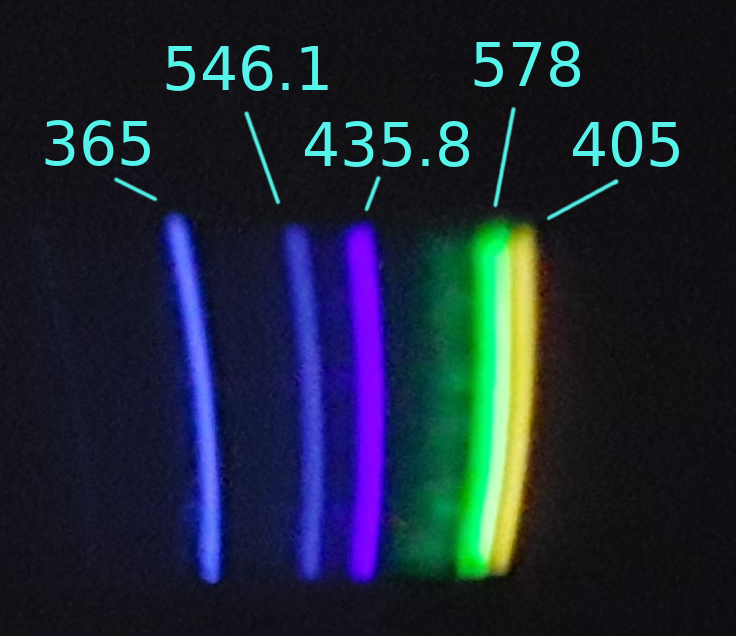
\includegraphics[width=.4\linewidth]{images/hg-spektrallinien.png}
    \caption{Spektrallinien der Hg-Dampf-Lampe}
    \label{fig:spektrallinien}
\end{figure}


Es  wurden  jeweils   die  Photospannung  und  die  Gegenspannung  der  f\"unf
spektrallinien   der   Hg-Dampf-Lampe   gemessen   und   in  den   Abbildungen
\ref{fig:photospannung}     und      \ref{fig:gegenspannung}      eingetragen.

\begin{figure}[H]
    \centering
    \begin{subfigure}{.45\linewidth}
        \centering
        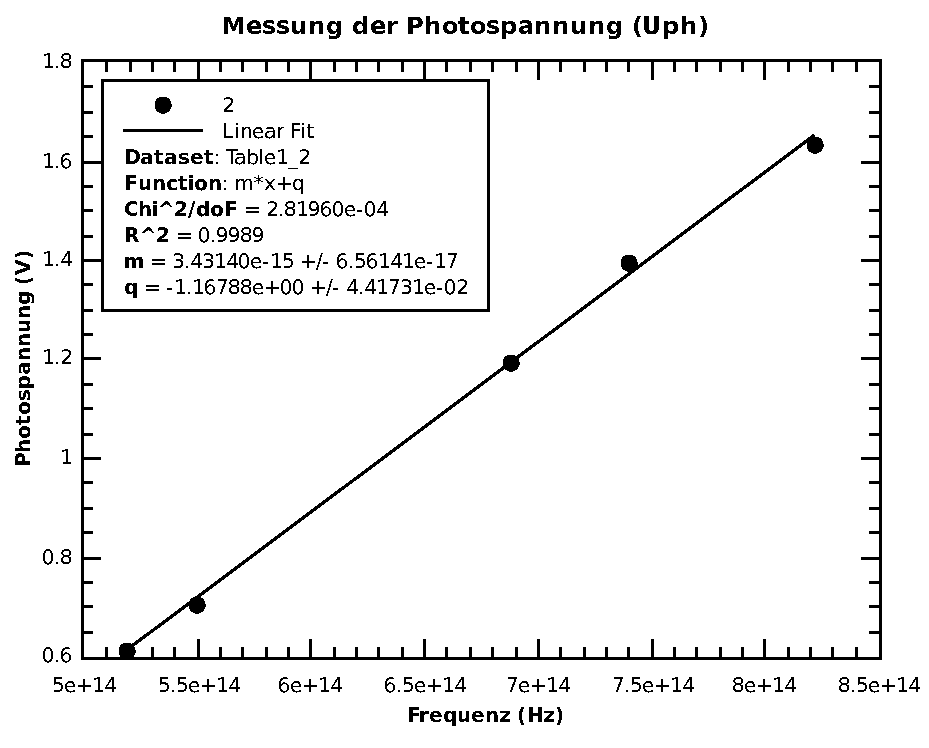
\includegraphics[width=\linewidth]{images/photospannung}
        \caption{Messung der Photospannung $U_{ph}$}
        \label{fig:photospannung}
    \end{subfigure}
    \begin{subfigure}{.45\linewidth}
        \centering
        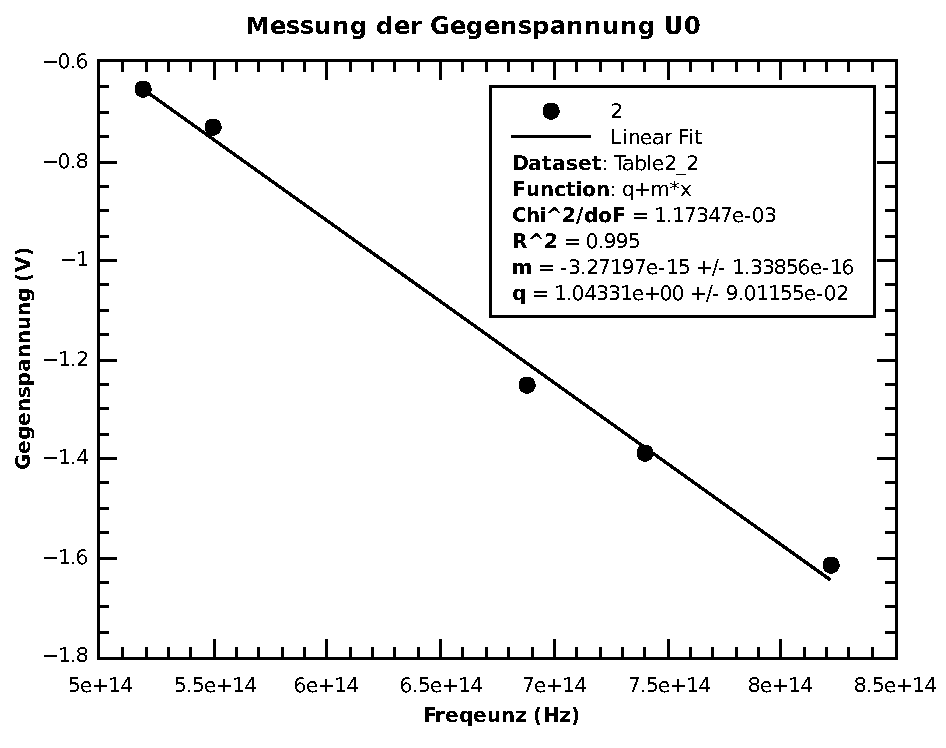
\includegraphics[width=\linewidth]{images/gegenspannung}
        \caption{Messung der Gegenspannung $U_0$}
        \label{fig:gegenspannung}
    \end{subfigure}
\end{figure}

Aus  einer  linearen  Regression werden die Steigungen gewonnen. Dabei ist  zu
beachten,  dass die Wellenl\"ange in \textbf{\SI{}{\nano\meter}} ist,  weshalb
wir die Steigung  nochmals mit dem Faktor $1e9$ multiplizieren. Das Vorzeichen
ist dabei egal. Die Steigungen sind:

\begin{align*}
    m_{ph} &= 4755830 \pm 274470 \\
    m_0    &= 4555350 \pm 183240
\end{align*}

\clearpage

In der zweiten  Messung  wurden  verschiedene  LEDs  an  einer  oszillierenden
Spannung   gelegt  und  eine  Spannungs-Strom  kennlinie  aufgenommen   (siehe
Abbildung \ref{fig:knickspannung-plot}. Die  Knickspannung  $U_k$  kann daraus
bestummen werden, siehe Abbildung \ref{fig:knickspannung}

\begin{figure}[H]
    \centering
    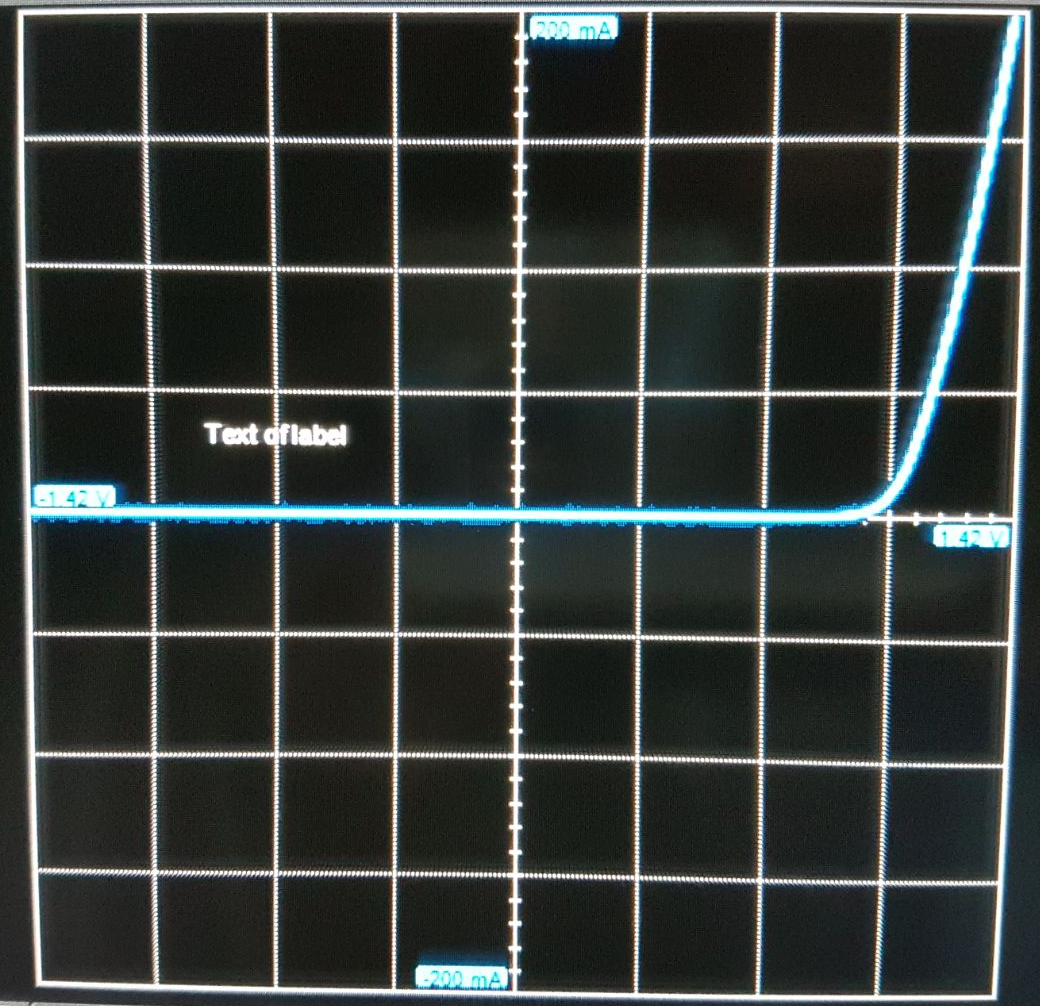
\includegraphics[width=.5\linewidth]{images/knickspannung.png}
    \caption{Messung der Knickspannung eines LEDs}
    \label{fig:knickspannung-plot}
\end{figure}

\begin{figure}[H]
    \centering
    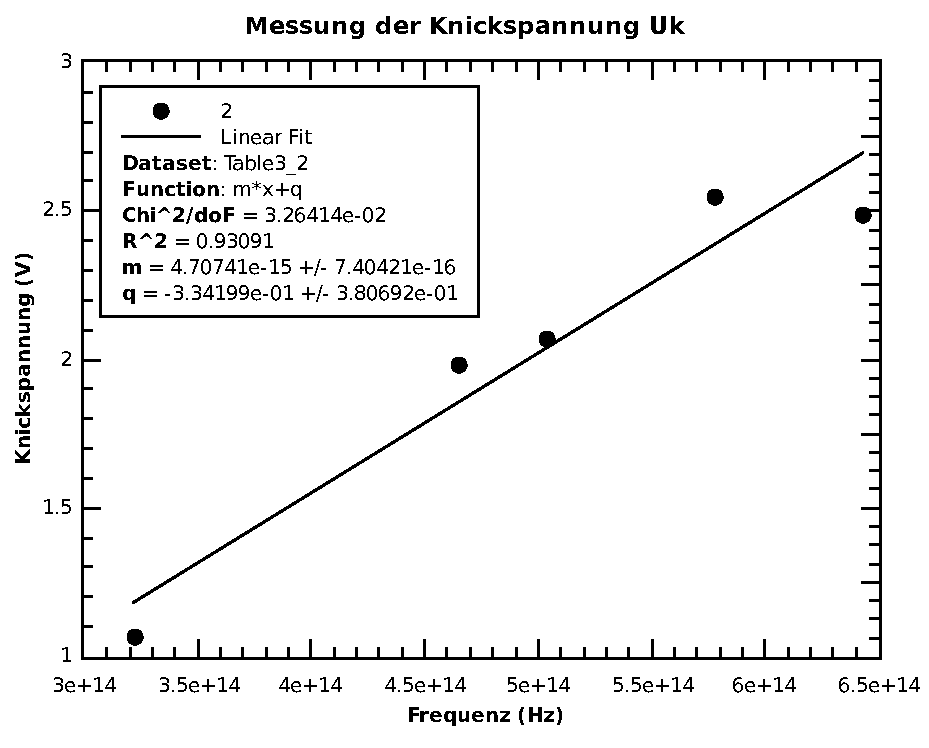
\includegraphics[width=.5\linewidth]{images/knickspannung.pdf}
    \caption{Messung der Knickspannung verschiedener LEDs}
    \label{fig:knickspannung}
\end{figure}

Wieder ist dabei zu beachten,  dass  die  Wellenl\"ange  in \SI{}{\nano\meter}
ist,  weshalb  die  Steigung  mit  dem  Faktor  $1e9$  multipliziert wird. Die
Steigung ist:

\begin{equation}
    m_{k} = 3239870 \pm 301223
\end{equation}

